%=========================================================================
% (c) 2011, 2012 Josef Lusticky

\chapter{System time support}
%\begin{figure}
	%\centering
	%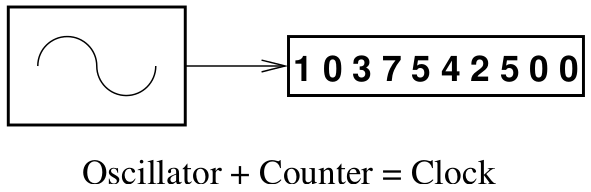
\includegraphics[width=6cm,keepaspectratio]{fig/clock.png}
	%\caption{Clock by P. Kamp}
	%\label{fig:hw-clock}
	%%\bigskip
%\end{figure}
For keeping, measuring and resolving time computer needs a clock.
Computer clock is an electronic device that counts oscillations in a
quartz crystal oscillator with a particular frequency~\cite{thesis-sync}.
These clocks are essentially timers associated with a counter register and
are capable of generating hardware interrupts.
The counter register counts the oscillations of the crystal.
When the counter registers reaches a specific value,
an interrupt is generated.
Such interrupt is called a {\it{clock tick}} (or {\it{timer tick}}) and at each clock tick,
interrupt service routine increments a system clock value stored in memory~\cite{thesis-sync}.

\section{Keeping and providing the time}\label{sec:system-keeping-and-providing}
The original IBM PC did know what time it was, provided you typed it in when you booted it,
but it forgot when you turned it off~\cite{timecounters}.
Today desktop computers %with CPU based on Intel x86 architecture
have hardware Real-Time Clock (RTC) in CMOS chip that is battery powered,
so it keeps time when the computer is powered off~\cite{timecounters}.
Hardware Real-Time Clocks should not be confused with the system clock,
which is a software system clock maintained by
the kernel and used to implement calls for getting the time,
as well as setting timestamps on files, etc~\cite{linux-man-rtc}.
The system clock will often be set to the current time using an RTC at boot time~\cite{linux-man-rtc},
so the systems without an RTC need to set the system clock another way,
such as across the network using NTP.

The kernel maintains then the current time and advances it at every interrupt.
The structure of the clock hardware of
typical desktop PCs is shown in figure~\ref{fig:system-pc-clock}.
An oscillator generates clock pulses that drive a counter~C.
Every time the counter reaches the value of a programmable latch~L,
an interrupt is generated and the counter is reset.
In a typical computer clock design, interrupts are produced at
fixed tick intervals in the range 1-20~ms~\cite{nanokernel}.
At each of these ticks the kernel then increases the internal variable
(usually called {\it{ticks}} or {\it{jiffies}}), which simply counts clock ticks,
as well as the variable, which represents the current system time~\cite{thesis-beat}.
Because of the speed requirement,
the system time use a linear time scale like seconds
(instead of dealing with seconds, minutes, hours, days, etc.)
and only if a human is in need of the current time,
the system time is converted~\cite{ntp-faq}.

\begin{figure}
  \centering
  
\includegraphics[width=9cm,keepaspectratio]{fig/pc-clock.png}
  \caption{PC clock hardware by R. Koster}
  \label{fig:system-pc-clock}
  %\bigskip
\end{figure}

The current system time can be queried via a system call
(traditionally called {\it{gettimeofday}}).
If it would simply return the value of the system time,
just the accuracy of the timer interrupt frequency could be provided.
However, this call may also query the hardware counter~C that is used for
interrupt generation and includes the time passed since
the last update of system time~\cite{thesis-beat}.

There are many possible hardware configurations among desktop computers today,
that an operating system can use as a hardware clock for a real-time support -
Programmable Interval Timer,
Time Stamp Counter register or High Precision Event Timer.
However, the concept described above applies to all of them.

In recent years a new design called {\it{tickless}} or {\it{dynamic ticks}}
has been in development~\cite{kernel-timer-systems}.
This allows an operating system kernel to run without a regular timer tick.
Such design is not used by Contiki OS~\cite{contiki-docs} and
therefore not further discussed in this thesis.

\section{Clock quality factors}
Unfortunately all the common clock hardware is not very accurate~\cite{ntp-faq}.
This is simply because the frequency that makes time increase is never exactly right.
Even an error of only 0.001\% would make a clock be off by almost one second per day.
Almost every clock can have an unique behaviour depending on many conditions~\cite{ntp-faq}.
The following factors are therefore used for expressing clock quality and behaviour:
\begin{itemize}
\item
Frequency is the rate at which a clock progresses~\cite{thesis-sync}.
\item
It is sometimes convenient
to express frequency offsets in parts-per-million~(PPM), where~1~PPM
is equal to $10^{-6}$ $\frac{s}{s}$ (0.0001\%)~\cite{rfc5905}.
\item
From long-term observation one may also notice variations in the clock frequency.
The difference of the frequency is called wander~\cite{ntp-faq}.
There can be clocks with poor short-term stability, but with good long-term stability, and vice versa.
\item
Resolution is the smallest possible increase of time the clock model allows.
If a clock increments its value only once per second, its resolution is also one second~\cite{ntp-faq}.
\item
Precision is the smallest possible increase of time that can be experienced
by a program~\cite{ntp-faq}.
\item
When repeatedly reading the time, the difference may vary almost randomly.
The difference of these differences (second derivation) is called jitter~\cite{ntp-faq}.
\item
Accuracy determines how close is the clock to an official time reference~\cite{ntp-faq}.
\item
Offset is the difference between the time read by the clock and the reference time~\cite{thesis-sync}.
\item
Reliability determines the time a clock can keep within a specified accuracy~\cite{ntp-faq}.
\end{itemize}

As mentioned before, all of the common hardware clock is not very accurate.
Real clocks have a frequency error of several PPM quite frequently
and some of the best clocks available still have errors of about $1^{-8}$PPM~\cite{ntp-faq}.
Even if the systematic error of some clock model is known, the clock will never be perfect.
This is because the frequency varies over time, mostly influenced by temperature,
but it could also be air pressure or magnetic fields~\cite{ntp-faq}.

\section{Clock corrections}
For keeping an accurate time a clock not only needs to be read, it must be also set.
However, simply setting the clock to remove the offset would cause unpredictable time steps~\cite{ntp-faq}.
Since time is an always monotonically increasing function, this is not a desired behaviour~\cite{}.
For minimising the time offset and frequency difference between
the reference clock and the local clock without any time step,
an NTP client can be used.

With the current system time knowledge,
the NTP client can compute an amount of adjustments needed for local clock
to get the local clock syncronised.
For accounting these adjustments
operating system must also provide a call
for adjusting the time (usually called {\it{adjtime}}).
This call speeds up or slows down the system time to be synchronised.
... TODO

%- software:
The Kernel Discipline -  kernel clock model RFC 1589 -
struct timex -
new calls ntp\_gettime, ntp\_settime, ntp\_adjtime

%However, some clock implementations do not allow small corrections to be applied to the system clock, and there is no standard interface to monitor the system clock's quality.
%=> divide problem (in RFC)
